%%%%%%%%%%%%%%%%%%%%%%%%%%%%%%%%%%%%%%%%%%%%%%%%%%%
%% Éléments flottants
%%%%%%%%%%%%%%%%%%%%%%%%%%%%%%%%%%%%%%%%%%%%%%%%%%%
%%%%%%%%%%%%%%%%%%
\section{Méthodologie de gestion du projet}
\subsection{Introduction}
\subsection{Étude préliminaire}
\subsubsection{Origine du génie logiciel}
\subsubsection{Comparaison des différents méthodes de développement}
\subsubsubsection{Les approches traditionnelles}
\subsubsubsection{Les méthodes agiles}
\subsubsubsection{Synthèse}
\subsection{Conduite de projet}
\subsubsection{Modèle de livraison}
Aujourd'hui, Cegedim adopte une démarche de livraison agile que chaque projet doit suivre. Le schéma ci-dessous montre les différentes phases de ce processus.
\begin{figure}[H]
    \begin{center}
        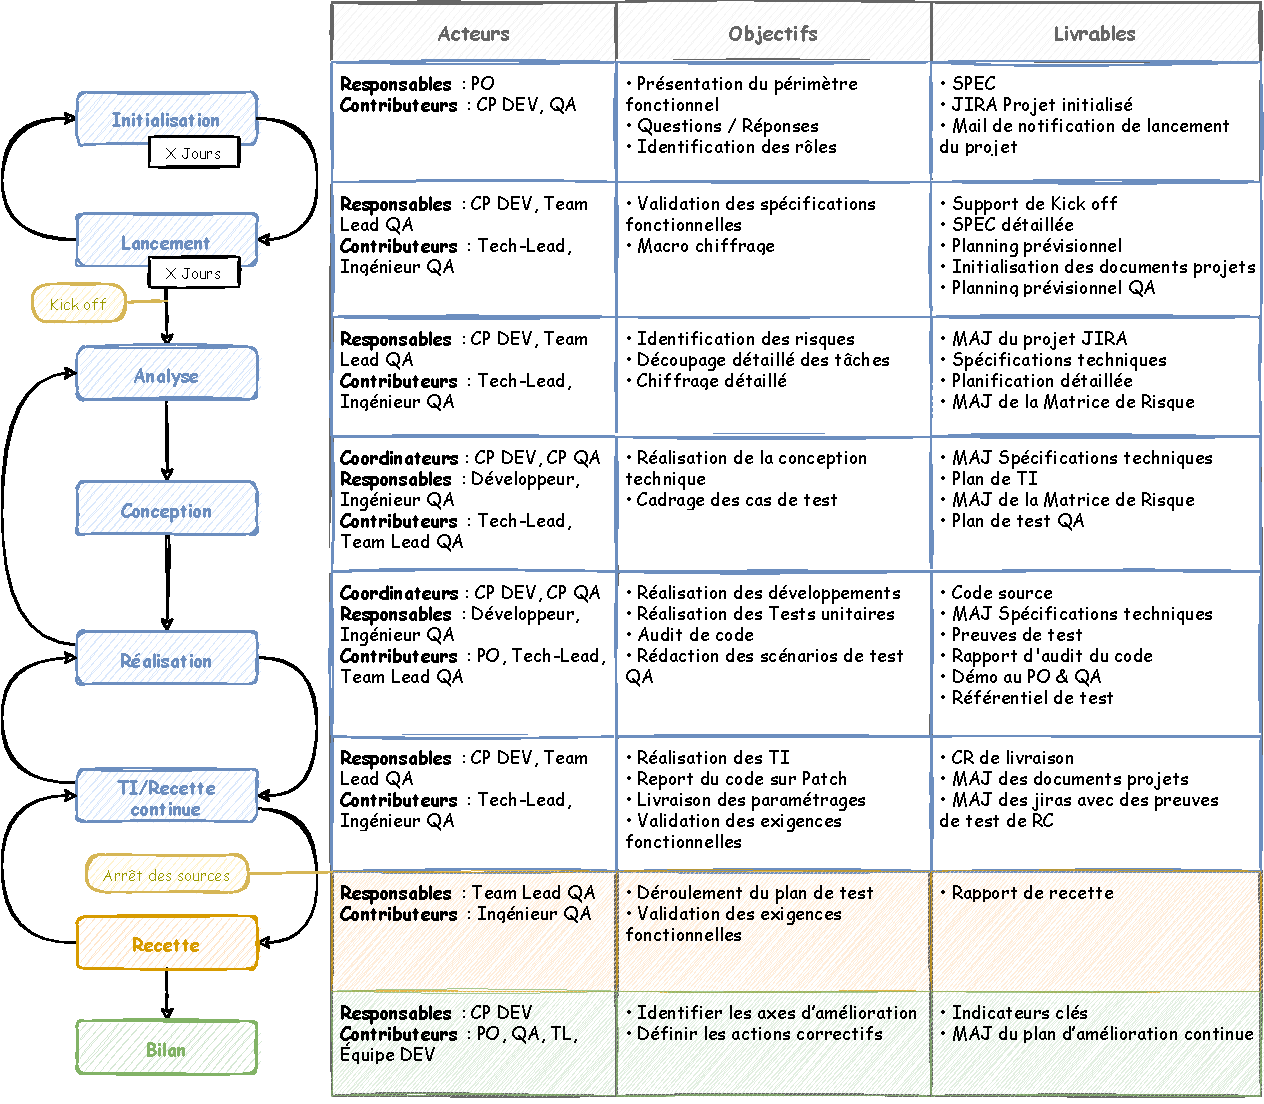
\includegraphics[width=\linewidth]{images/sec3/deliveryprocess.pdf}
        \caption{Processus de livraison }
    \end{center}
\end{figure}
\subsubsection{Déroulement du projet}
scrum
retrospective 
sprint
\subsubsection{Processus de développement}
specs fonctionnelles
codage
test unitaire
audit de code
documentation
\subsubsection{Gestion du workflow git}
Le workflow de travail pour les branches GIT choisi au niveau de Cegedim SRH est Gitflow. Git Flow est un modèle de dépôt git permettant d'améliorer les processus de développement et de mise en production d'un projet.\\
Voici un schéma présentant l'organisation du dépôt git ainsi que les différentes interactions qu'il peut y avoir entre chaque branche :
\subsection{Planification et suivi du projet}
\subsubsection{Diagramme de Gantt}
Le diagramme de gantt:\\
\begin{figure}[H]
    \begin{center}
        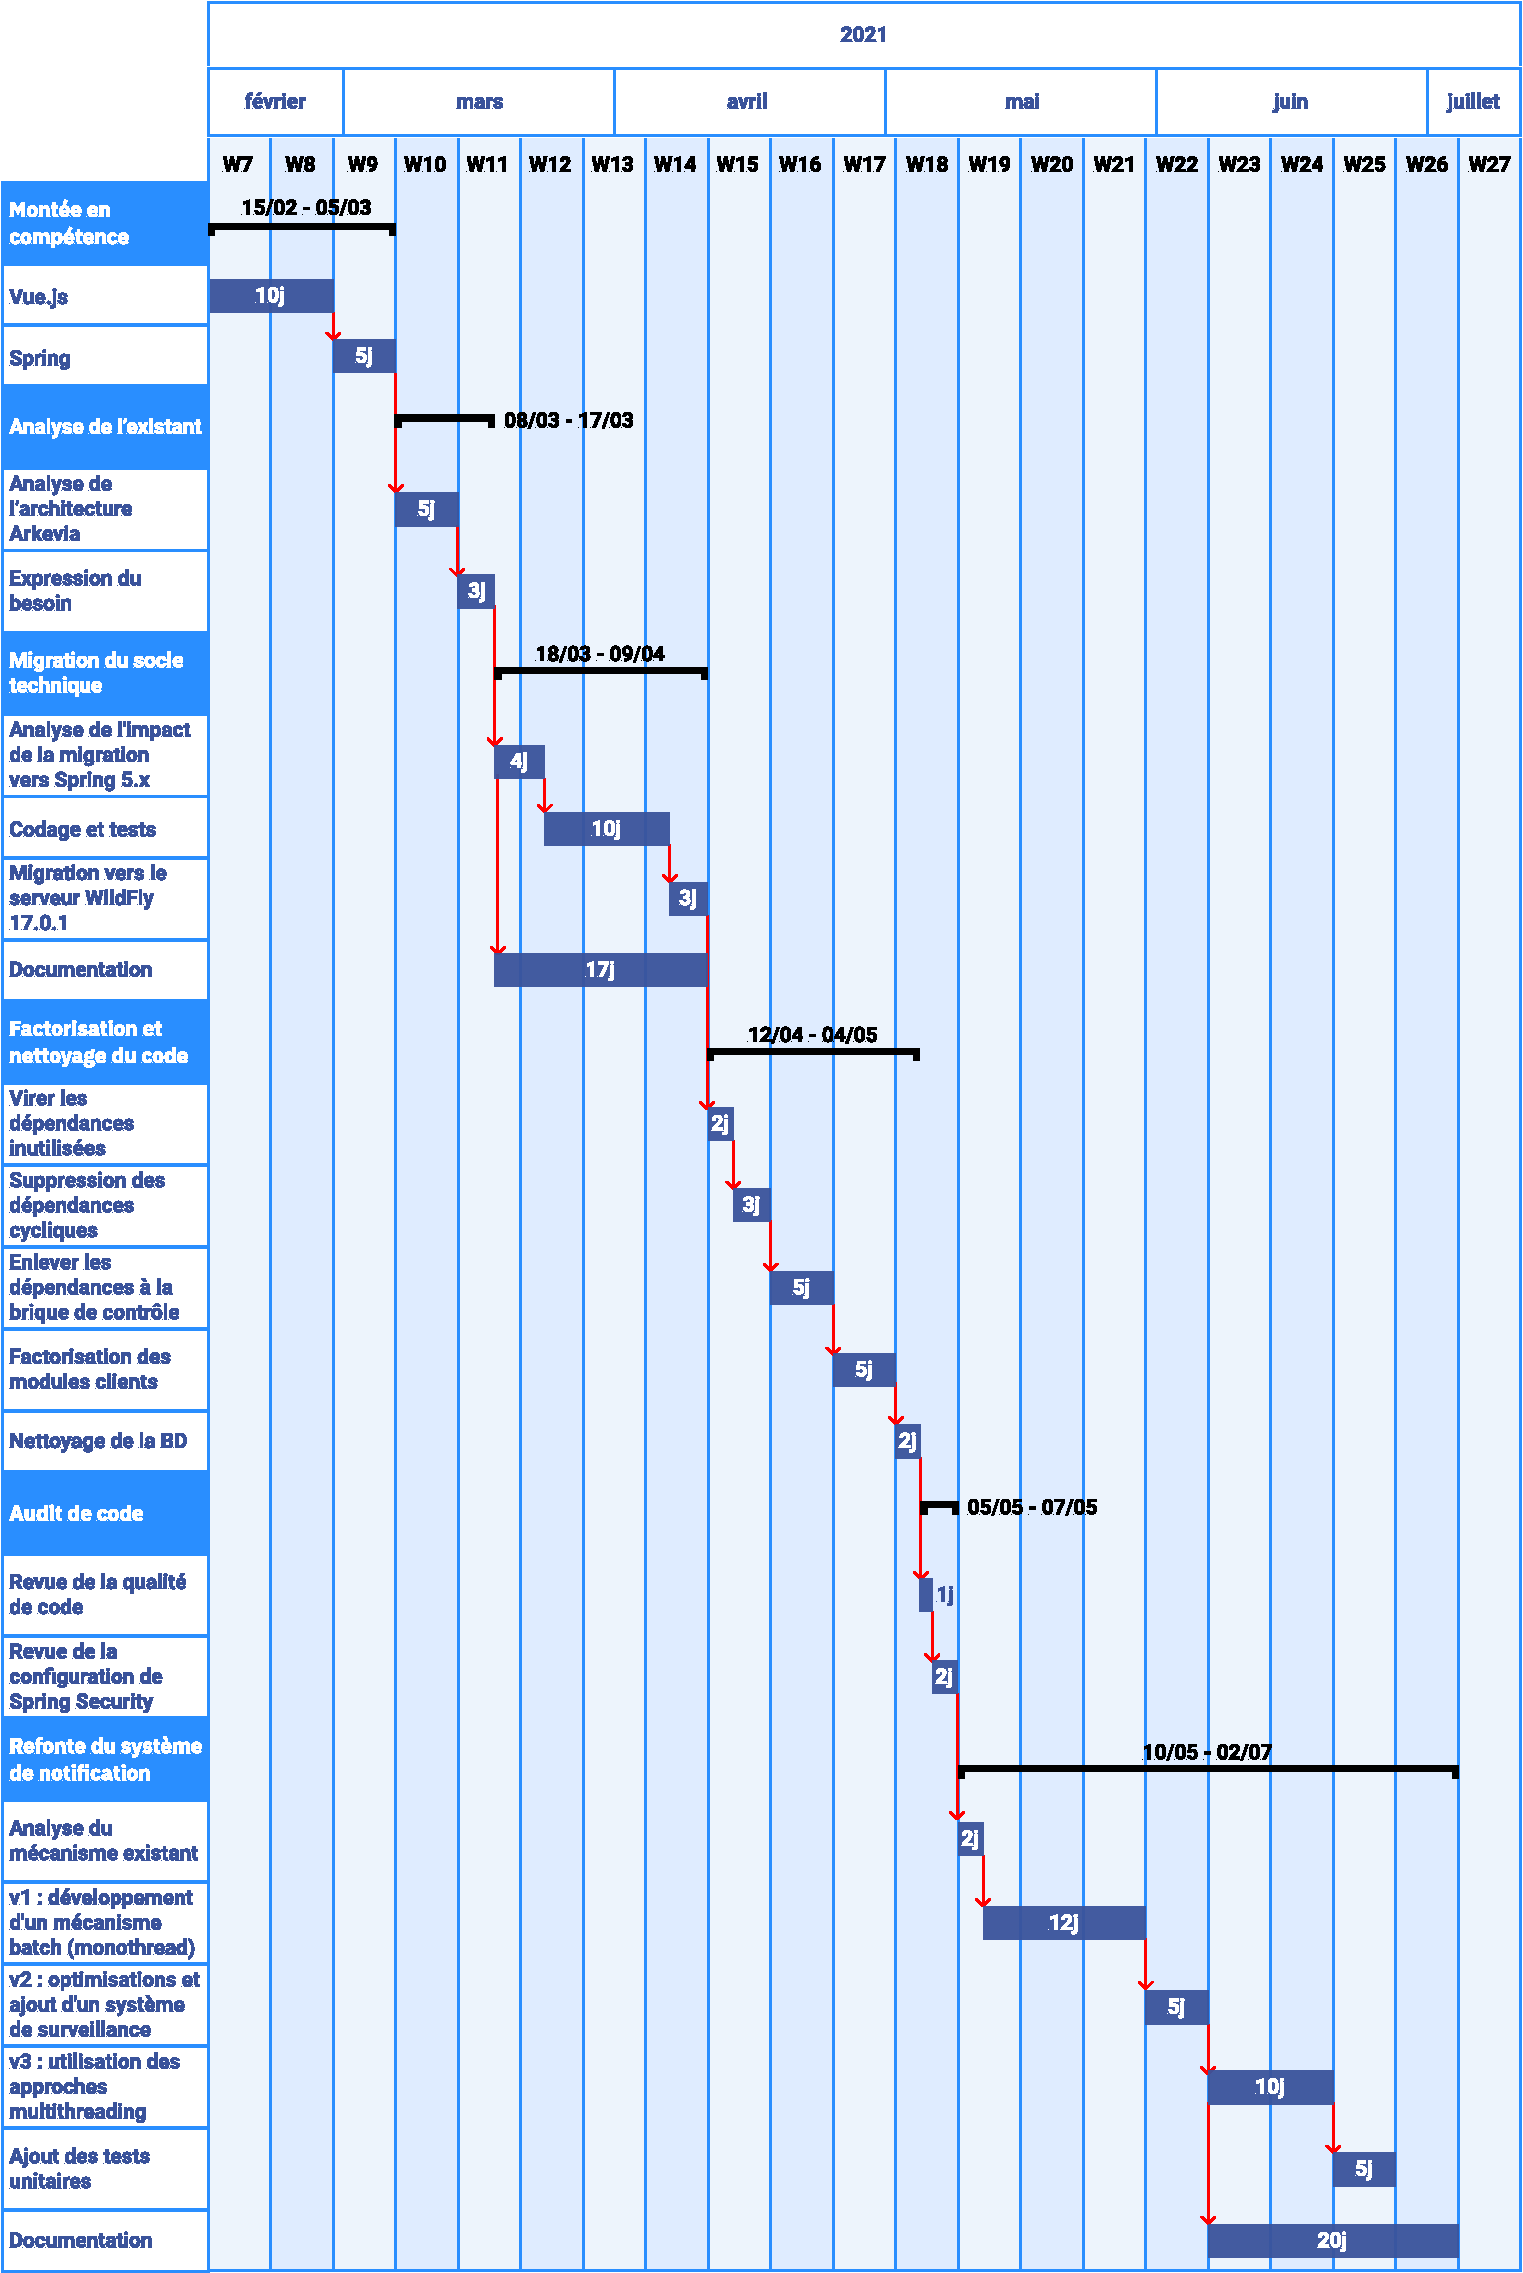
\includegraphics[width=\linewidth]{images/sec3/gantt.pdf}
        \caption{Diagramme de Gantt}
    \end{center}
\end{figure}
\subsection{Conclusion}
%%%%%%%%%%%%%%%%%%
